%%%%% Physik Kompendium Nr.2 %%%%%
%% 04 -- Erläuterungen zum Wechselstromkreis %%



\subsection{Grundlegende Begriffe}		\label{subsec:ErlaeuterungenGrundlegend}


\subsubsection{Wechselstrom}

Wechselstrom bezeichnet die einen Strom der nicht nur von einem Punkt zum Anderen fließt, sondern mit einer Frequenz die Fließrichtung wechselt. Obwohl am Ende unter dem Strich keine Elektronen vollständig \glqq übergelaufen\grqq{} sind, wird trotzdem Energie verbraucht.

Typischerweise weißt die Spannungskurve den Verlauf der Sinuskurve auf.


\subsubsection{Amplitude}

Ist die maximale Auslenkung der Spannung oder der Stromstärke, also der Scheitelwert der Sinuskurve. Oft mit $\hat{U}$ bzw. $\hat{I}$ oder $U_{0}$ bzw. $I_{0}$ angegeben.


\subsubsection{Frequenz}

Bezeichnet die Anzahl Perioden pro Zeiteinheit. \\ Einheit ist $Hz$, also $\frac{1}{T}$, wobei $T$ die Zeit für eine Periode ist.


\subsubsection{Periode}

Dauer, bis eine volle Sinuskurve der Spannung vollendet ist, also die Spannung wieder den Nullpunkt aus der selben Richtung passiert, wie beim ersten Durchlauf.

Bei einem Wechselstromgenerator (siehe Sektion \ref{sec:Generator} auf Seite \pageref{sec:Generator}) ist dies die Dauer, bis sich die Spule um 360\degree gedreht hat.


\subsubsection{Winkelgeschwindigkeit}

Zeit pro Winkel. Im \textbf{Bogenmaß} (Taschenrechner bei Winkeln umstellen!) berechnet mit:

\begin{equation}	\label{eq:Winkelgeschwindigkeit}
	\omega = \frac{2\pi}{T} = 2\pi f
\end{equation}



\subsection{Weitere Begriffe}	\label{subsec:ErlaeuterungenWeitere}

\subsubsection{Effektive Spannung}

Diese beschreibt die durchschnittliche Spannung, die zum weiteren Rechnen wie eine Spannung im Gleichstromkreis behandelt werden kann.

Für eine Sinuskurve lässt sie sich wie folgt, in Abhängigkeit der maximalen Spannung, berechnen:

\begin{equation}	\label{eq:EffektiveSpannung}
	U_{eff}=\frac{\hat{U}}{\sqrt{2}}
\end{equation}


\subsubsection{Effektive Stromstärke}

Diese beschreibt die durchschnittliche Stromstärke, die zum weiteren Rechnen wie eine Stromstärke im Gleichstromkreis behandelt werden kann.

Für eine Sinuskurve lässt sie sich wie folgt, in Abhängigkeit der maximalen Stromstärke, berechnen:

\begin{equation}	\label{eq:EffektiveStromstaerke}
	I_{eff}=\frac{\hat{I}}{\sqrt{2}}
\end{equation}


\subsubsection{Phasenverschiebung}

Eine Phasenverschiebung ist die x-Achsen-Verschiebung einer Kurve, typischerweise der Sinus-Kurve des Stroms. Sie wird in Grad und relativ zur Kurve der Spannung angegeben.\footnote{Illustration von \url{http://upload.wikimedia.org/wikipedia/commons/d/db/Phasenverschiebung_kapazitiv.svg}}

\begin{figure}[h!]
	\centering
	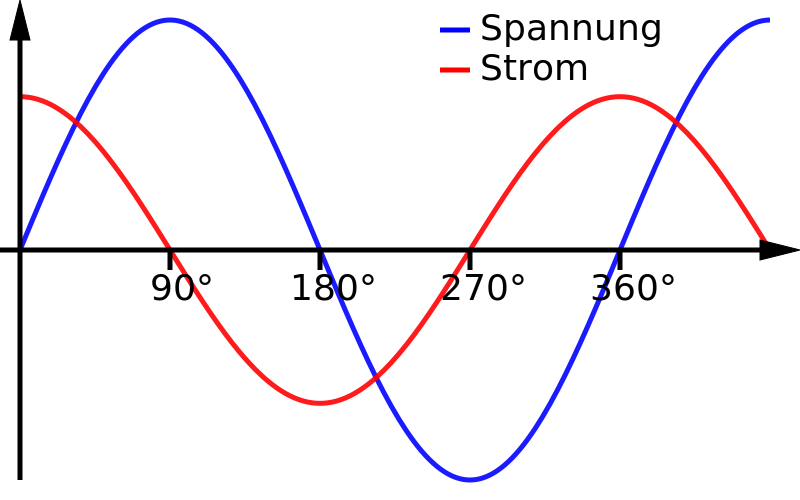
\includegraphics[width=0.5\textwidth]{Pictures/Phasenverschiebung}
	\caption{\glqq Die Spannung eilt dem Strom voraus.\grqq }
\end{figure}


\subsubsection{Impedanz}

Die Impedanz $Z$ ist der Gesamtwiderstand im Wechselstromkreis, die sich durch den Quotienten aus der Spannung und der Stromstärke berechnen lässt:

\begin{equation}		\label{eq:Impedanz}
	Z = \frac{U_{eff}}{I_{eff}}
	  = \frac{\hat{U}}{\hat{I}}
\end{equation}


\subsubsection{Kapazitiver Widerstand}

Für den kapazitiven Widerstand $X_C$, der von Kondensatoren im Wechselstromkreis ausgeht, siehe Sektion \ref{subsec:KapazitiverWiderstand} auf Seite \pageref{subsec:KapazitiverWiderstand}.


\subsubsection{Induktiver Widerstand}

Für den induktiven Widerstand $X_C$, der von Spulen im Wechselstromkreis ausgeht, siehe Sektion \ref{subsec:InduktiverWiderstand} auf Seite \pageref{subsec:InduktiverWiderstand}.






